%%%%%%%%%%%%%%%%%%%%%%%%%%%%%%%%%%%%%%%%%%%%%%%%%%%%%%%%%%%%%%%%%%
\chapter{Related work aka what's the current situation}

% =============================================================================
\section{Previous Work}
maybe describe the software cartography prototype?

% =============================================================================
\section{Related Work}


Using \MDS to visualize information based on the metaphor of cartographic maps is by no means a novel idea. \emph{Topic maps}, as they are called, have a longstanding tradition in information visualization \cite{Ware04a}. The work in this paper was originally inspired by Michael Hermann's and Heiri Leuthold's work on the political landscapes of Switzerland \cite{Herm03a}. 

In the same way, stable layouts have a long history in information visualization, as a starting point see \eg the recent work by Frishman and Tal on online dynamic graph drawing \cite{Fris08a}. They present an online graph drawing approach, which is similar to the online pipeline presented in this work. Please refer to \autoref{sec:other} for a comparison of graph drawing and \MDS. 

ThemeScape is the best-known example of a text visualization tool that uses the metaphor of cartographic maps. 
Topics extracted from documents are organized into a visualization where visual distance correlates to topical distance and surface height corresponds to topical frequency \cite{Wise95b}. The visualization is part of a larger toolset that uses a variety of algorithms to cluster terms in documents. For laying out small document sets MDS is used; for larger document sets a proprietary algorithm, called ``Anchored Least Stress'', is used. The digital elevation model is constructed by successively layering the contributions of the contributing topical terms, similar to our approach.

In the software visualization literature however, topic maps are rarely used.
Except for the use of graph splatting in RE Toolkit by Telea \etal \cite{Tele03a}, we are unaware of their prior application in software visualization. And even in the case of the RE toolkit, the maps are not used to produce consistent layouts for thematic maps, or to visualize the evolution of a software system. 

\begin{figure}
\begin{center}
  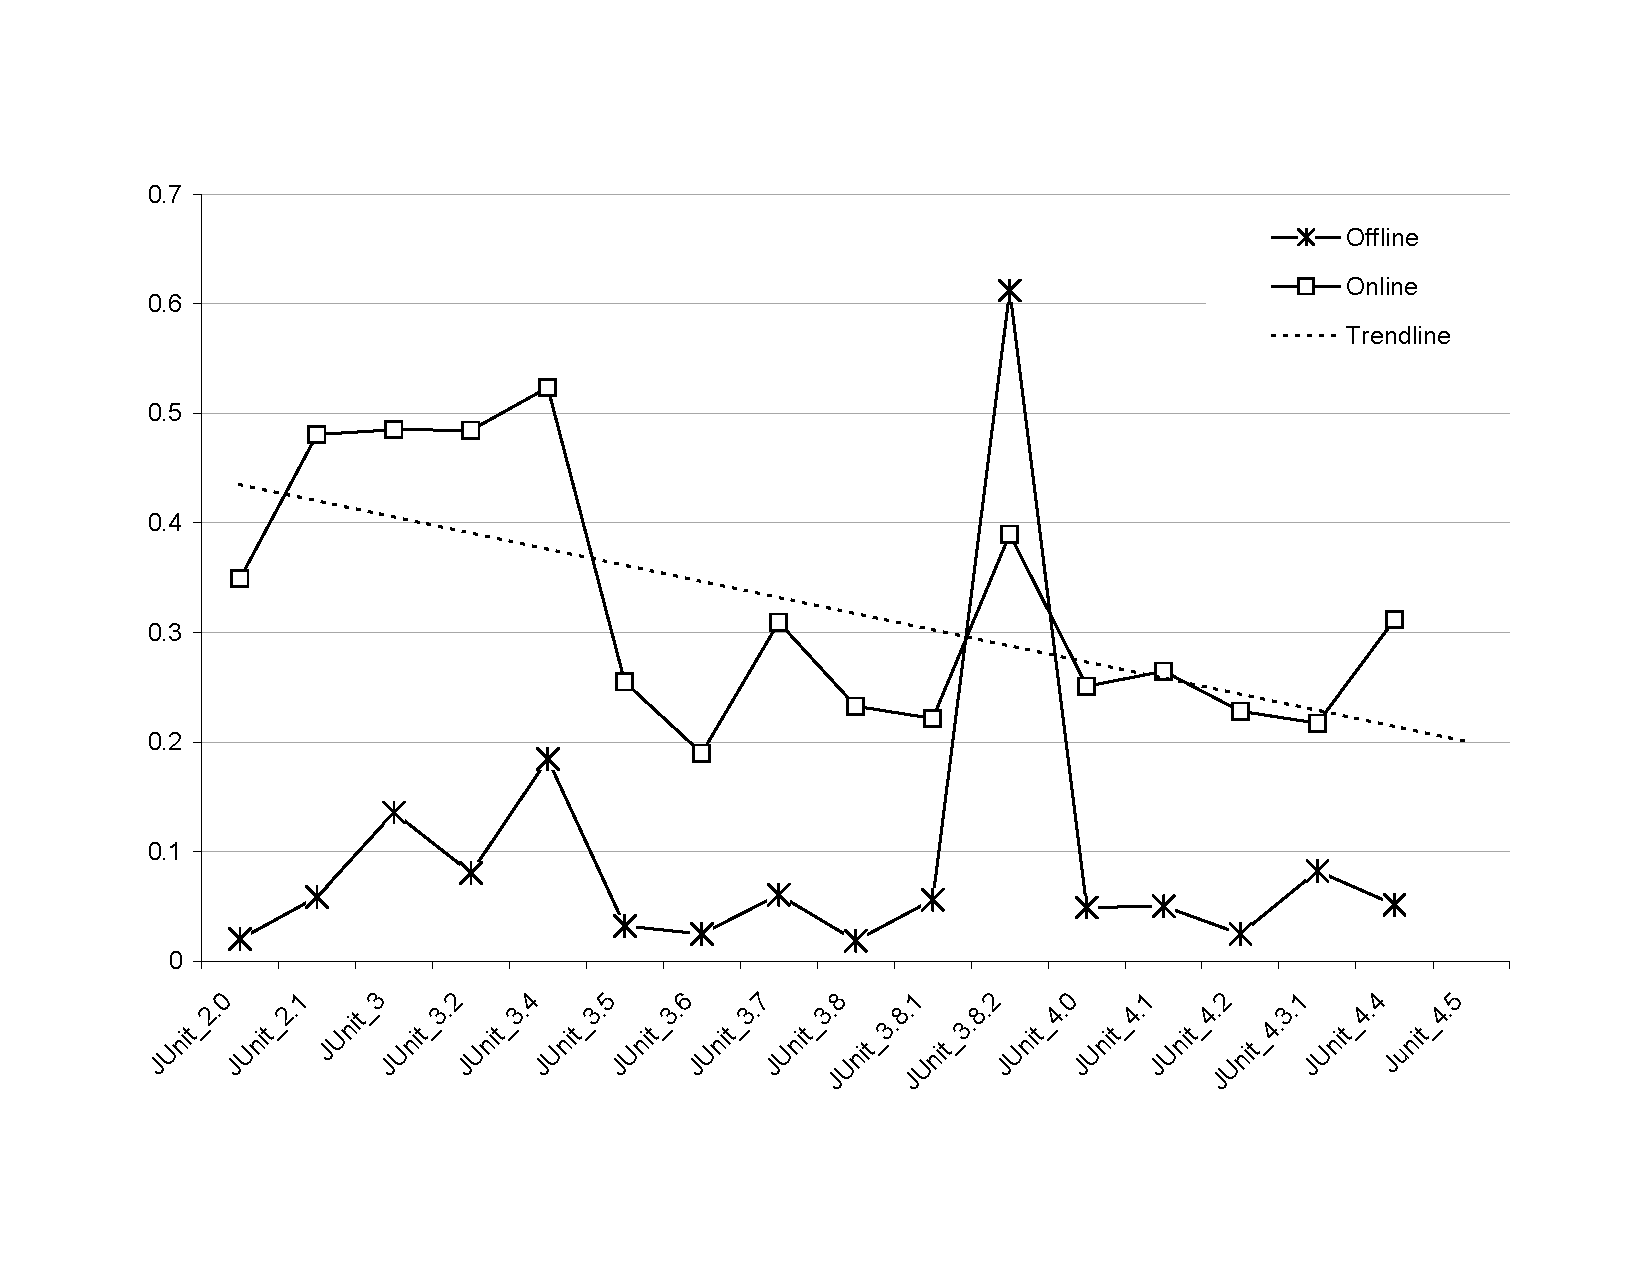
\includegraphics[width=0.7\linewidth]{junitchart.pdf}
\end{center}
    \caption{Stability chart of JUnit: the peak between release 3.8.2 and release 4.0 originates from the removal of the SwingUI classes and the addition of annotation processing classes. The online stability trends towards the offline stability.}
    \label{fig:junitchart}
\end{figure}

\begin{figure}
\begin{center}
  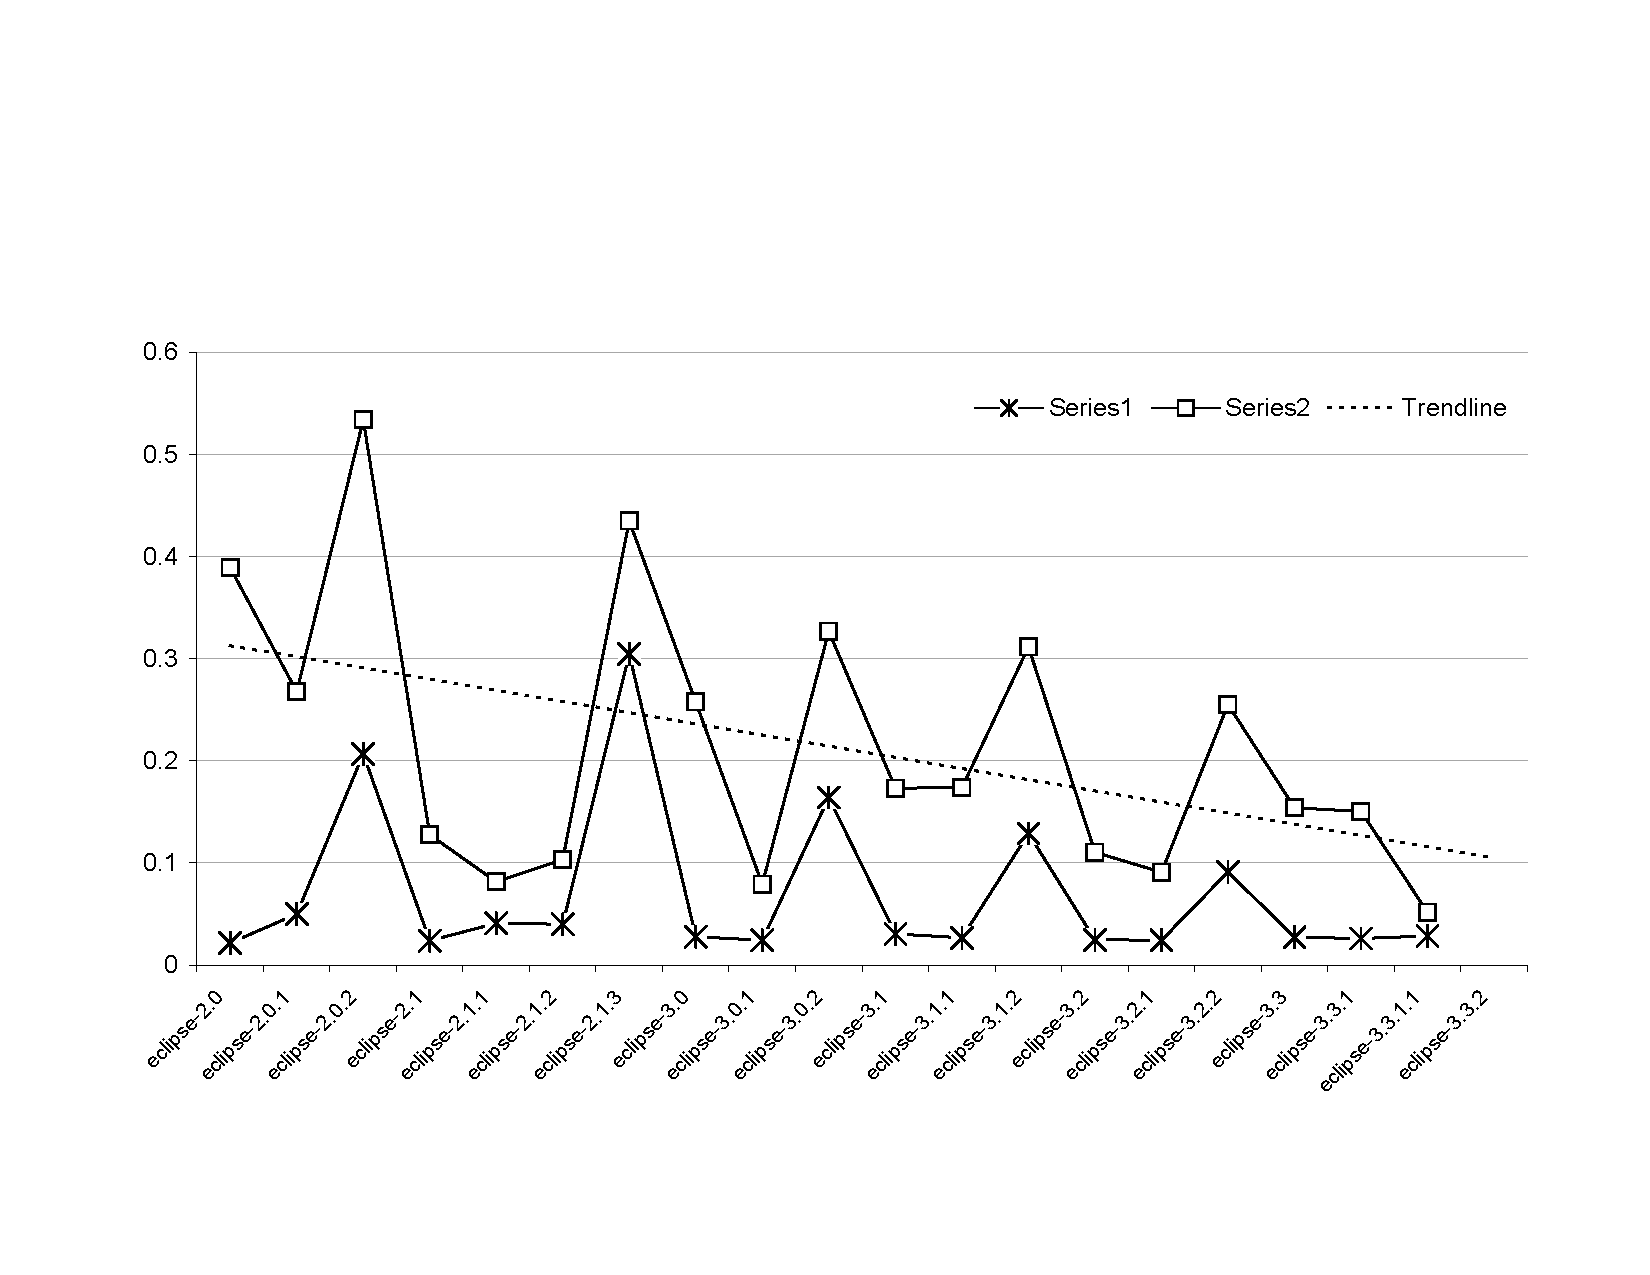
\includegraphics[width=0.85\linewidth]{eclipsechart.pdf}
\end{center}
    \caption{Stability chart of Eclipse: There are five peaks of instability, each of them correlates with a major release (\ie release 2.1. release 3.0, release 3.1, release 3.2, and release 3.3). The online stability trends towards the offline stability.}
    \label{fig:eclipsechart}
\end{figure}


\subsection{Desiderata for Spatial Representation of Software}

Robert DeLine's work on software navigation \cite{Deli05b,Deli06a} closely relates to \SOCA. His work is based on the observation that developers are consistently lost in code \cite{Deli05a} and that using textual landmarks only places a large burden on cognitive memory. He concludes the need for new visualization techniques that allow developers to use their spatial memory while navigating source code.

DeLine proposes four desiderata \cite{Deli05b} that should be satisfied by spatial software navigation: 1)~the display should show the entire program and be continuous, 2)~the display should contain visual landmarks such that developers can find parts of the program perceptually rather than relying on names, 3)~the display should remain visually stable during navigation [and evolution], and 4)~the display should be capable of showing global program information overlays other than navigation.

An ad-hoc algorithm that satisfies the first and fourth properties is presented in the same work. As distance metric between software entities (here, methods) an arbitrary chosen score is used.

Our work satisfies all above desiderata, and completes them with a fifth desideratum that visual distance should have a meaningful interpretation. The scope of \SOCA is broader than just navigation, it is also intended for reverse engineering and code comprehension in general. We can thus generalize the five desiderata for spatial representation of software as follows:

\begin{enumerate}
\item The visualization should show the entire program and be continuous.
\item The visualization should contain visualization landmarks that allow the developers to find parts of the system perceptually, rather than relying on name or other cognitive causes. 
\item The visualization should remain visually stable as the system evolves. 
\item The visualization should should be capable of showing global information overlays.
\item On the visualization, distance should have a meaningful interpretation. 
\end{enumerate}


% ~~~~~~~~~~~~~~~~~~~~~~~~~~~~~~~~~~~~~~~~~~~~~~~~~~~~~~~~~~~~~~~~~~~~~~~~~~~~~
\subsection{Other Layout Approaches used in Software Visualization}

Most software visualization layouts are based on one or multiple of the following approaches: UML diagrams, force-based graph drawing, tree-map layouts, and polymetric views.

% -------------------------------------
\emph{UML diagrams} generally employ no particular layout and do not continuously use the visualization pane. The UML standard itself does not cover the layout of diagrams. Typically a UML tool will apply an unstable graph drawing layout (\eg based on visual optimization such a reducing the number of edge crossings) when asked to automatically layout a diagram. However, this does not imply that the layout of UML diagrams is meaningless. UML diagrams are carefully created by architects, at least those made during the design process, so their layout do have a lot of meaning. If you change such a diagram and re-show it to its owner, the owner will almost suddenly complain, since he invested time in drawing the diagram a certain way! Alas, this layout process requires manual effort.

Gudenberg \etal have proposed an evolutionary approach to layout UML diagrams in which a fitness function is used to optimize various metrics (such as number of edge crossings) \cite{Gude06a}. Although the resulting layout does not reflect a distance metric, in principle the technique could be adapted to do so. Andriyevksa \etal have conducted user studies to assess the effect that different UML layout schemes have on software comprehension \cite{Andr05a}.
They report that the layout scheme that groups architecturally related classes together yields best results. They conclude that it is more important that a layout scheme convey % NB: "convey", not "conveys" (subjunctive)
a meaningful grouping of entities, rather than being aesthetically appealing. Byelas and Telea highlight related elements in a UML
% Google says 51,700 x an UML and 315,000 a UML %
diagram using a custom ``area of interest'' algorithm that connects all related elements with a blob of the same color, taking special care to minimize the number of crossings \cite{Byel06a}.
The impact of layout on their approach is not discussed.

% -------------------------------------
\emph{Graph drawing} refers to a number of techniques to layout two- and three-dimensional graphs for the purpose of information visualization \cite{Ware04a,Kauf01b}. Noack \etal offer a good starting point for applying graph drawing to software visualization \cite{Noac05a}. Jucknath-John \etal present a technique to achieve stable graph layouts over the evolution of the displayed software system \cite{Juck06a}, thus achieving consistent layout, while sidestepping the issue of reflecting meaningful position or distance metrics.

Unlike MDS, graph drawing does not map an $n$-dimensional space to two dimensions, rather it is concerned with the placement of vertices and edges such that visual properties of the output are optimized. For example, algorithms minimize the number of edge crossings or try to avoid that nodes overlap each other. Even though, the standard force-based layouts can consider edge weights (which can be seen as a distance metric), edges with the same weight may have different length on the visualization pane depending on the connectedness of the graph at that position. Furthermore, the resulting placement is not continuos. The void between vertices is not continuous spectrum of metric locations, as is the case with an MDS layout.

\emph{Graph splatting} is a variation of graph drawing, which produced visualizations that are very similar to thematic maps \cite{Lier03a}. Graph splatting represents the layout of graph drawing algorithms as a continuous scalar field. Graph splatting combines the layout of graph drawing with the rendering of thematic maps. Each vertex contributes to the field with a Gaussian shaped basis function. The elevation of the field thus represents the density of the graph layout at that position. Telea \etal apply Graph splatting in their RE toolkit to visualize software systems \cite{Tele03a}. However, they are not concerned with stable layouts. Each run of their tool may yield a different layout.

% -------------------------------------
\emph{Treemaps} represent tree-structured information using nested rectangles \cite{Ware04a}.
Though treemaps make continuous use of the visualization pane, the interpretation of position and distance is implementation dependent. Classical treemap implementations are known to produce very narrow and thus distorted rectangles. Balzer \etal proposed a modification of the classical treemap layout using Voronoi tessellation \cite{Balz05a}. Their approach creates aesthetically more appealing treemaps, reducing the number of narrow tessels. There are some treemap variations (\eg the strip layout or the squarified layout) that can, and do, order the nodes depending on a metric. However, nodes are typically ordered on a local level only, not taking into account the global co-location of bordering leaf nodes contained in nodes that touch at a higher level. Many treemaps found in software visualization literature are even applied with arbitrary order of nodes, such as alphanumeric order of class names. 

\emph{Polymetric views} visualize software systems by mapping different software metrics on the visual properties of box-and-arrow diagrams \cite{Lanz03d,Lanz06a}. Many polymetric views are ordered by the 
value of a given software metric, so that relevant items appear first (whatever first means, given the 
layout). Such an order is more meaningful then alphabetic (or worse, hash-key ordering), but on the other hand only as stable as the used metric. The System Complexity view is by far the most popular polymetric view, and is often used as a base layout where our requirements for stability and consistence apply (see \eg \cite{Gree06a}). The layout of System Complexity uses graph drawing on inheritance relations, and orders the top-level classes as well as each layer of subclasses by class names. Such a layout does not meet our desiderate for a stable and consistent layout.
   
% ~~~~~~~~~~~~~~~~~~~~~~~~~~~~~~~~~~~~~~~~~~~~~~~~~~~~~~~~~~~~~~~~~~~~~~~~~~~~~
\subsection{ More Cartography Metaphors in Software Visualization}\label{sec:other}

A number of tools have adopted metaphors from cartography in recent years to visualize software.
Usually these approaches are integrated in a tool with in an interactive, explorative interface and often feature three-dimensional visualizations. None of these approaches satisfies DeLine's desiderata.

MetricView is an exploratory environment featuring UML diagram visualizations \cite{Term05a}. The third dimension is used to extend UML with polymetric views \cite{Lanz03d}.
The diagrams use arbitrary layout, so do not reflect meaningful distance or position.

White Coats is an explorative environment also based on the notion of polymetric views \cite{Mesn05b}. The visualizations are three-dimensional with position and visual-distance of entities given by selected metrics. However they do not incorporate the notion of a consistent layout.

CGA Call Graph Analyser is an explorative environment that visualizes a combination of function call graph and nested modules structure \cite{Bohn07a}. The tool employs a 2$\frac{1}{2}$-dimensional approach. To our best knowledge, their visualizations use an arbitrary layout.

CodeCity is an explorative environment building on the city metaphor \cite{Wett07b}. CodeCity employs the nesting level of packages for their city's elevation model, and uses a modified tree layout to position the entities, \ie packages and classes. Within a package, elements are ordered by size of the element's visual representation. Hence, when changing the metrics mapped on width and height, the overall layout of the city changes, and thus, the consistent layout breaks.

VERSO is an explorative environment that is also based on the city metaphor \cite{Lang05a}. Similar to CodeCity, VERSO employs a treemap layout to position their elements. Within a package, elements are either ordered by their color or by first appearance in the system's history. As the leaf elements have all the same base size, changing this setting does not change the overall layout. Hence, they provide consistent layout, however within the spatial limitations of the classical treemap layout. 
